\section{Question 5}
L’algorithme de branch-and-bound est représenté à la figure~\ref{arbre5}.

\begin{figure}[htb]
	\caption{Algorithme par séparation et évaluation, branch and bound}
	\label{arbre5}
	\centering
	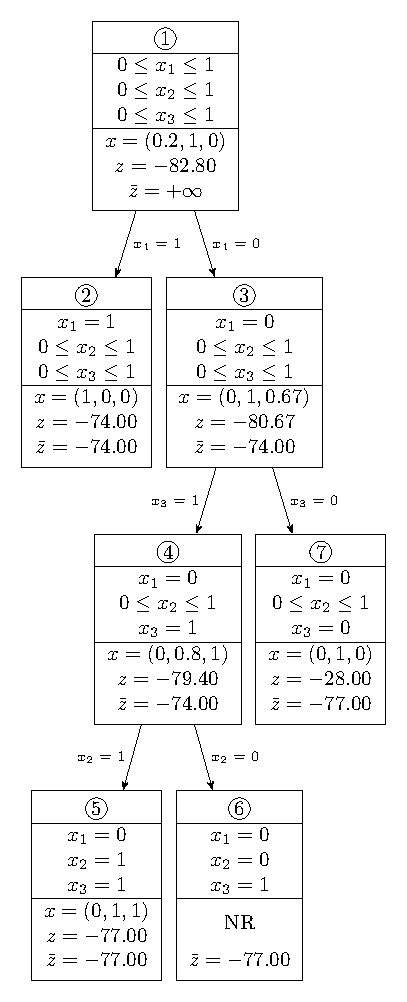
\includegraphics[height=.98\textheight]{question/forest/5.pdf}
\end{figure}

La solution optimale \Circled{1} est $x = (0.2, 1, 0)$ et la valeur de la fonction à minimiser est égale à $-82.80$. Étant donné que $x$ n’est pas une solution entière et que $x_1$ est la seule valeur non entière, nous allons appliquer une contrainte sur sur $x_1$. Soit $x_1 = 1$ , soit $x_1 = 0$. En contraignant $x$ à être égale à 1, on trouve une solution entière : $x = (0.2, 1, 0)$ \Circled{2}. Le meilleur minimum avec une solution passe ainsi de $+\infty$ (pas de solution) à $-74.00$. Étant donné qu’on a trouvé une solution entière, on arrête l’exploration de cette branche pour passer à la contrainte $x_1 = 0$x. Sur cette branche, on trouve une nouvelle solution $x = (0, 1, 0.67)$ \Circled{3}. $x_3$ étant la seule valeur non entière de la solution on va appliquer la contrainte à cette variable. Et ainsi de suite. Il y a trois raisons pour lesquelles on peut arrêter l’exploration d’une branche :
\begin{itemize}
	\item la solution n’est pas réalisable \Circled{6};
	\item la solution est entière \Circled{2} \Circled{5} \Circled{7};
	\item la solution prend une valeur supérieure à une solution entière déjà trouvée ($z \geq \bar{z}$) : cela ne sert à rien d’explorer la branche plus en avant, toutes les solutions entières trouvées seront moins optimales que l’actuelle meilleure solution entière.
\end{itemize}